\vspace{40px} \section{Modulated signal spectrum}
The spectrum analysis is helpful for a better understanding of the behavior of the BPSK modulation technique. Analyzing the spectrum provides insights into the distribution of signal power across different frequencies. In this section, there will be the analysis an the plots of a periodic \texttt{1010} sequence and a randmoly generated sequence.

% as we can see we don't see the carrier component on the center of the graph. 

% beacause when we sbtract the two cbask the component subtract there but the other two components adds ip because of the oppsoite phases. We have twice as much for the amplitude shif key,ng (energy redistribuition for BPSK)



\subsection{Periodic \texttt{1010} sequence signal}
To analyze and plot the spectrum of a periodic \texttt{1010} sequence signal some important values should be calculated. The $\omega_0$ value, which is the angular carrier frequency, the value, representing the base harmonic frequency and $k$, which is the range in which the spectrum will be calculated. The first two values may be calculated with the following expression:

\begin{equation*}
    \omega_0 = 2\pi f_0 \hspace{30px} \Omega = \frac{\pi}{\tau}
\end{equation*}

\noindent The $k$ range is a range of $n$ indexes around the carrier frequency central index, $k_0 = \frac{\omega_0}{\Omega}$. These values can be easily obtained by running the below-displayed code snippet.

\begin{lstlisting}
    % anguolar carrier frequency
    omega_0 = 2 * pi * f0; 

    % base harmonic angoular frequency 
    OMEGA = pi / tau; 

    % Carrier frequency central index
    k_0 = omega_0 / OMEGA;

    % Define range of indexes for spectrum
    k = k_0 + (-10 : 10);
\end{lstlisting}

\noindent At this point, the BPSK spectrum can be calculated. To do so it is necessary to calculate the Fourier series coefficient for the BASK\footnote{Which stands for Binary Amplitude Shift Keying} modulation type using the following equation:

\begin{equation*}
    C_{BASK}(k) = j\frac{U}{4} \frac{\sin\left[ \left( k\Omega - \omega_0 \right) \frac{\tau}{2}\right]}{\left( k\Omega - \omega_0 \right) \frac{\tau}{2}}
\end{equation*}

\noindent Now that the BASK coefficients are calculated, the BPSK coefficients are easy to be computed:

\begin{equation*}
    C_{BPSK}(k) = C_{BASK}(k) \left[ e^{+jk\Omega\frac{\tau}{2}} - e^{-jk\Omega\frac{\tau}{2}} \right]
\end{equation*}

\noindent These two complex equations can be computed in MATLAB with the help of the \texttt{sinc} function as follows:

\begin{lstlisting}
    % Phase value of the spectral function
    phase = (k * OMEGA - omega_0) * tau / 2;

    C_BASK = sinc(phase / pi) * U / 4 * 1j; % fourirer series coefficient, BASK

    % BPSK spectrum for periodocal '1' and '0' sequence (...1 0 1 0 1 0 1 0 1 0...)
    C_BPSK = C_BASK .* ( exp(1j * k * OMEGA * tau / 2) -  exp(- 1j * k * OMEGA * tau / 2));
\end{lstlisting}

\noindent The code for plotting the spectrum of the BPSK for a periodic sequence signal is shown below. 

\begin{lstlisting}
    % creates figure and settings
    f = figure(2);
    f.Name = 'Analysis of BPSK spectrum';
    f.NumberTitle = 'off';
    f.Position = [450, 100, 700, 600];
    
    % plot 1st result
    subplot(2, 1, 1), stem( k * OMEGA / (2 * pi), abs(C_BPSK), 'b' ), grid on,
    xlabel('Frequency [GHz]'), ylabel('Amplitude, [V]'), title('Amplitude Spectrum of periodic signal')
    ylim([-0.05, 0.35]);
\end{lstlisting}

\begin{figure}[h]
    \centering
    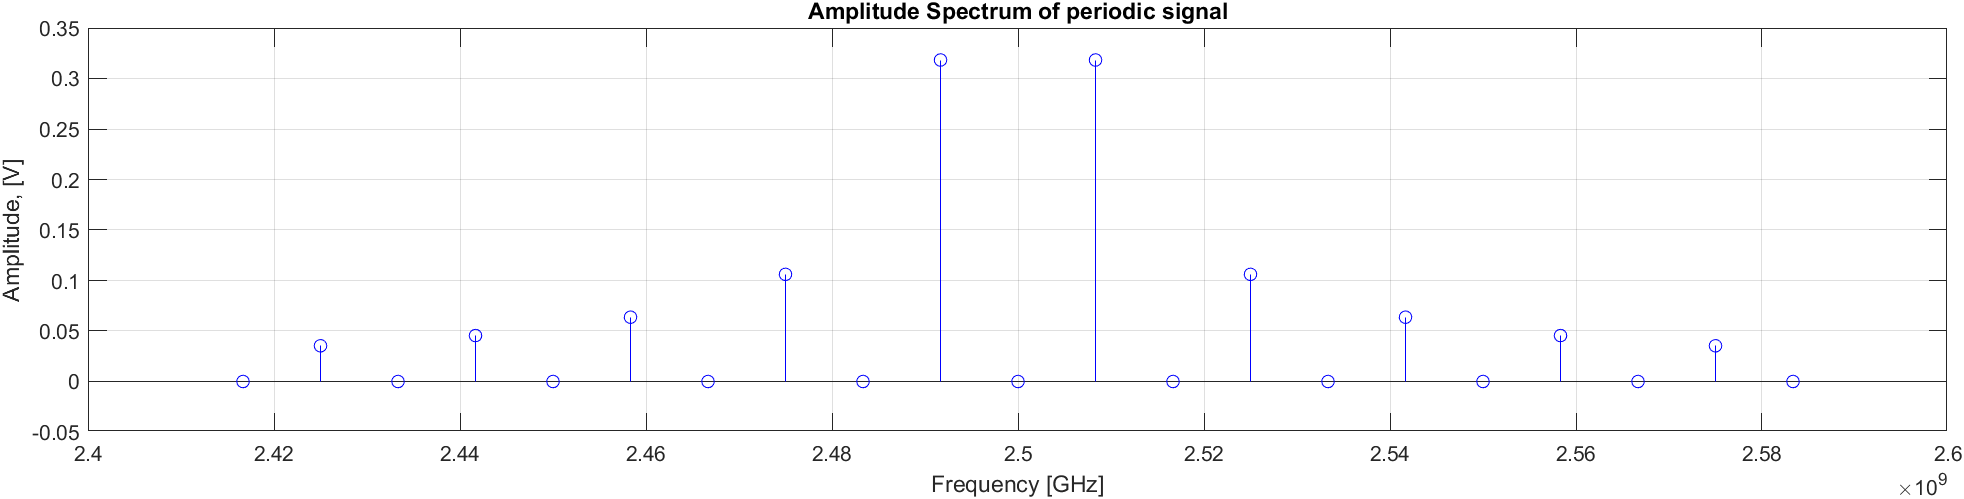
\includegraphics[width = \textwidth]{../res/imgs/periodic-signal-spectrum.png}
    \caption{BPSK periodic signal spectrum.}
    \label{fig:periodic-signal-spectrum}
\end{figure}


\subsection{Random sequence signal}

we have twice as great value compared for the BASK.


\begin{lstlisting}
    % Power Spectral Density (PSD) for random input signal
    omega = ( k(1) : 1/100 : k(end) ) * OMEGA; % angoular frequency 

    phase = (omega - omega_0 ) * tau / 2; % continuous phase 2

    S_BASK =  2 * tau * sinc(phase / pi ) * U / 4 * 1j;


    % PSD as a normalized squarred spectral function
    G_BPSK = 1/ tau * abs(S_BASK) .^2;


    subplot(2, 1, 2), plot( omega / (2 * pi), G_BPSK, 'b' ), grid on,
    xlabel('Frequency [GHz]'), ylabel('PSD'), title('PSD of random signal')
    ylim([-0.1e-8, 1.6e-8]);
\end{lstlisting}


\begin{figure}[h]
    \centering
    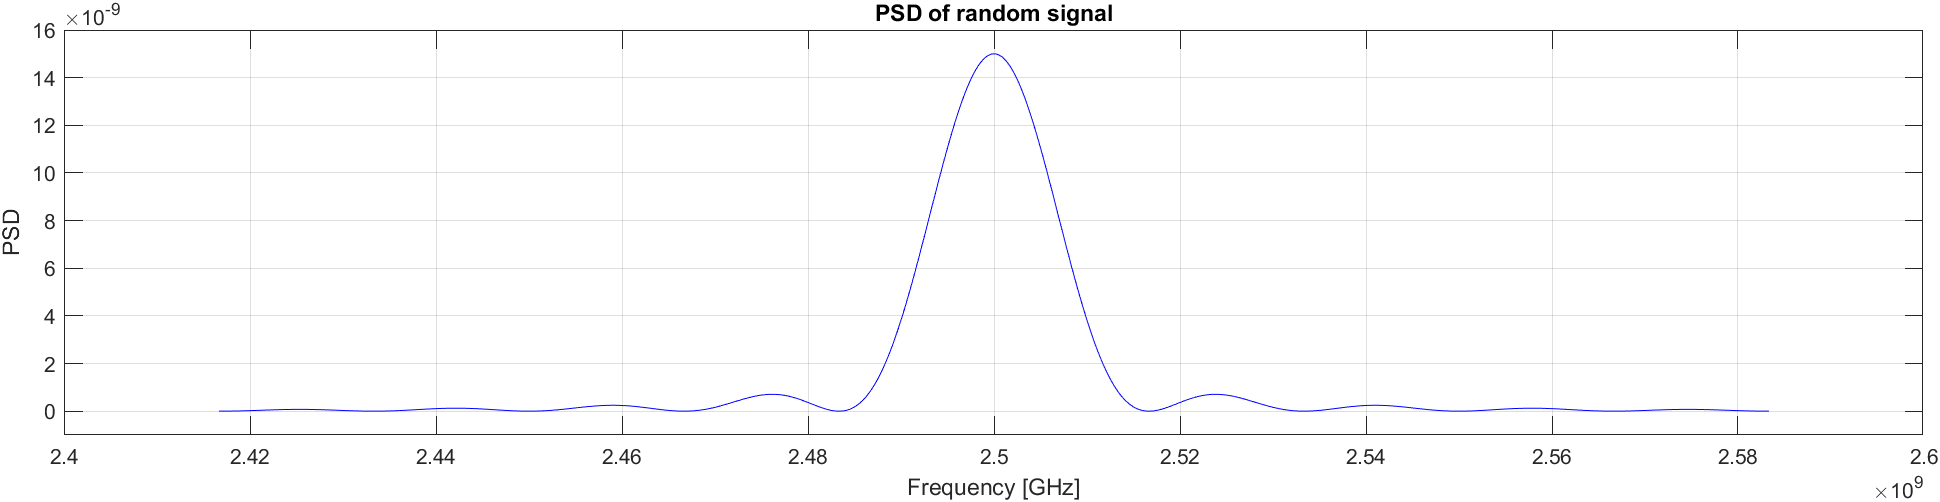
\includegraphics[width = \textwidth]{../res/imgs/random-signal-spectrum.png}
    \caption{BPSK random signal spectrum.}
    \label{fig:random-signal-spectrum}
\end{figure}